\chapter{Grundlagen}
\label{cha:grundlagen}
In dem Kapitel werden Anleitungen für die Installation von Emacs auf
ausgewählten Betriebssystemen gegeben. Es werden die Grundlagen von
Emacs beschrieben, um mit Konfigurationsdateien arbeiten zu können.\\

\section{Installation}
Emacs wird offiziell auf folgenden Systemen unterstützt \cite{Hahn2016}:
\begin{itemize}
\item Linux(alle Distributionen)
\item FreeBSD
\item NetBSD
\item OpenBSD
\item OS X auf Mac
\item Solaris
\item Microsoft Windows\\
\end{itemize}
Es folgen Anleitungen für die Installation auf \textit{Ubuntu
  18.04.1}\footnote{\url{http://releases.ubuntu.com/18.04/}},
\textit{macOs High
  Sierra}\footnote{\url{https://www.apple.com/at/macos/high-sierra/}}
und \textit{Microsoft Windows
  10}\footnote{\url{https://www.microsoft.com/de-at/windows}}. Die
Installation erfolgt bei allen drei Betriebssystemen anhand einer
Paketverwaltung, des {\glqq}package managers{\grqq}. Für
\textit{Windows 10} und \textit{macOs High Sierra} müssen diese
\textit{package manager} installiert werden. In jeder der Methoden
wird Emacs in der Version 25 installiert.\\

\subsection{Emacs unter Ubuntu Linux installieren}
Auf \textit{Ubuntu Linux} wird Emacs, mit der Hilfe des \textit{APT
  package
  managers}\footnote{\url{https://help.ubuntu.com/lts/serverguide/apt.html.en}}
installiert. Folgende Zeile muss in einem Terminal ausgeführt werden:
\begin{lstlisting}
sudo apt-get -y install emacs
\end{lstlisting}

\subsection{Emacs unter Mac Os High Sierra installieren}
Hier wird Emacs mittels
\textit{homebrew}\footnote{\url{https://brew.sh/index_de}}
installiert. Zum Installieren von Emacs folgende Zeilen in einem
Terminal ausführen, nachdem \textit{homebrew} installiert wurde:
\begin{lstlisting}
brew update
brew install emacs --with-cocoa
brew linkapps emacs
sudo rm /usr/bin/emacs
sudo rm -rf /usr/share/emacs
\end{lstlisting}

\subsection{Emacs unter Microsoft Windows installieren}
Für \textit{Windows} wird
\textit{chocolatey}\footnote{\url{https://chocolatey.org/}}
verwendet. Dazu muss die
\textit{Powershell}\footnote{\url{https://www.google.com/search?client=ubuntu&channel=fs&q=windows+powershell&ie=utf-8&oe=utf-8}}
als Administrator ausgeführt werden, nachdem \textit{chocolatey}
installiert wurde. Folgende Zeile muss ausgeführt werden:
\begin{lstlisting}
choco install -y emacs
\end{lstlisting}

\section{Strg und Alt}
In Emacs beginnen alle Tastenkombination mit der Strg-Taste oder der
Alt-Taste. Um die Tastenkombination in der Schreibweise möglichst kurz
zu halten, werden Abkürzungen verwendet. Die Strg-Taste, welche für
Steuerung steht und im Englischen für \textit{control}, wird als
{\glqq}C{\grqq} abgekürzt. Die Alt-Taste, welche für Alternative oder
im Englischen für \textit{alternate} steht, wird als {\glqq}M{\grqq}
für {\glqq}Meta-Key{\grqq} abgekürzt. Anstelle der Alt-Taste kann auch
die esc-Taste verwendet werden. \cite{Hahn2016}\\\\ Beispiele:
\begin{itemize}
\item \textbf{C-x C-f} = Strg-Taste gedrückt halten + x und danach
  Strg-Taste gedrückt halten + f
\item \textbf{M-x} = Alt-Taste gedrückt halten + x
\item \textbf{C-M-v} = Strg-Taste und Alt-Taste gedrückt halten + v\\
\end{itemize}

\section{Navigation}
Emacs ist grundsätzlich dafür ausgelegt, komplett ohne Benutzung der
Maus auszukommen. Dies resultiert in einem schnelleren
Editieren. Grundsätzlich kann mit den Pfeiltasten navigiert werden, um
den Zeiger in Emacs zu bewegen. Ist dabei die Strg-Taste gedrückt, so
werden bei den Pfeiltasten links und rechts ganze Wörter
übersprungen. Bei den Pfeiltasten auf und ab mit gedrückter
Strg-Taste, wird an das Ende, beziehungsweise den Anfang des Absatzes
gesprungen. Weiter nützliche Tastenkombinationen sind:
\begin{itemize}
\item C-a: Springe an den Anfang der Zeile.
\item C-e: Springe an das Ende der Zeile.
\item M-<: Springen an den Anfang des Puffers.
\item M->: Springen an das Ende des Puffers.
\end{itemize}
Die nachfolgende Grafik \ref{fig:Navigation} veranschaulicht die
Sprünge des Zeigers.\\

\begin{figure}[h]
  \centering
  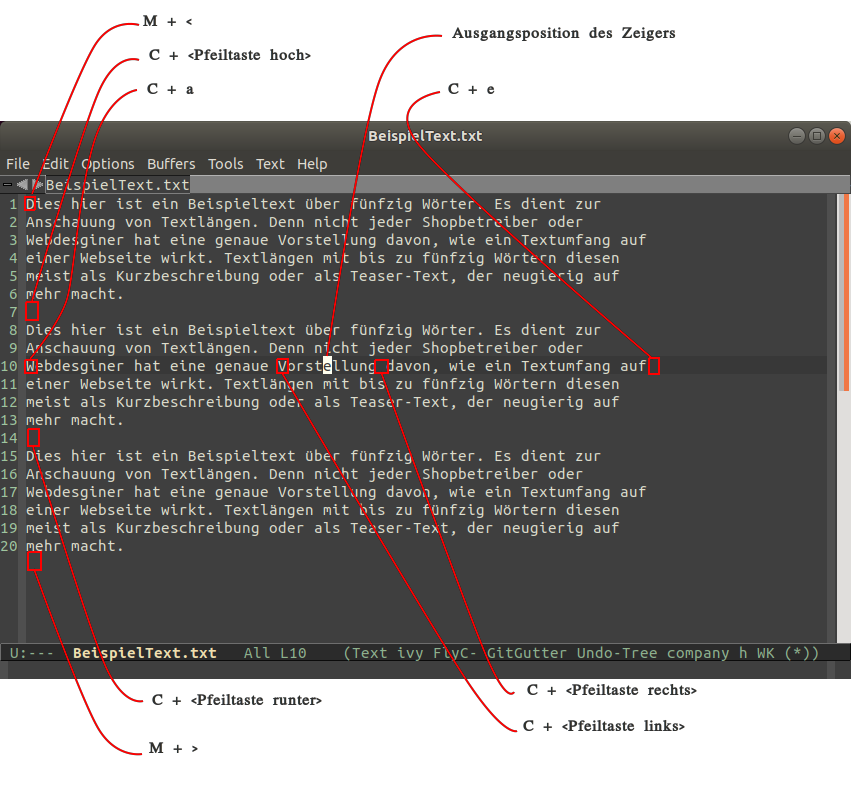
\includegraphics[width=.95\textwidth]{./images/Grundlagen/Navigation.png}
  \caption{\label{fig:Navigation} Diese Abbildung veranschaulicht die
    Sprünge des Zeigers mit unterschiedlichen Tastenkombinationen.}
\end{figure}
Um den sichtbaren Bereich des Textes zu verschieben, werden folgende
Tastenkombinationen verwendet:

\begin{itemize}
\item \textbf{C-v}: Seite nach oben {\glqq}verschieben{\grqq}.
\item \textbf{M-v}: Seite nach unten {\glqq}verschieben{\grqq}.
\item \textbf{C-l}: Mittiges Ausrichten der Seite bezogen auf die
  Position des Zeigers. Erneutes ausführen der Tastenkombination
  verschiebt die Zeile in der sich der Zeiger befindet an den oberen
  Rand des Bildschirms, danach an den unteren Rand und danach wieder
  in die Mitte.\\
\end{itemize}
Es gibt einige weitere Möglichkeiten um in Emacs zu navigieren. Dafür
stehen bereits eine Vielzahl an Tutorials zur Verfügung. Ein solches
ist das in Emacs enthaltene Tutorial. Dieses kann direkt in Emacs mit
der Tastenkombination \textbf{C-h t} aufgerufen
werden. \cite{CameronRosenblattRaymond1996}\\

\section{Hilfe}
Emacs hat eine eingebaute Hilfe. Die Tastenkombination für die Hilfe
ist: \textbf{C-h} gefolgt von einem weiteren Buchstaben. Mit der
Tastenkombination \textbf{C-h ?} wird die Hilfe für die Hilfe
aufgerufen. Hier wird alles über die Verwendung der Hilfe
erklärt. Beendet wird die Hilfe mittels
\textbf{C-g}. \cite{CameronRosenblattRaymond1996}\\\\ Weitere
hilfreiche Tastenkombinationen für die Hilfe sind:
\begin{itemize}
\item \textbf{C-h c}: Gibt den Namen der Funktion im
  \textit{minibuffer} (siehe Abschnitt \ref{sec:emacsstart}) aus,
  welche für die eingetippte Tastenkombination ausgeführt wird.
\item \textbf{C-h k}: Beschreibt die Funktion, die hinter der
  eingetippten Tastenkombination steckt.
\item \textbf{C-h f}: Beschreibt die eingetippte Funktion.
\item \textbf{C-h v}: Beschreibt die eingetippte Variable.\\
\end{itemize}

\section{Puffer}
\label{sec:puff}
Wird in Emacs ein Text editiert, so geschieht dies in Emacs in einem
Puffer. Wenn eine Datei geöffnet wird, dann wird der Text von Emacs in
einem Puffer gehalten. Beim Start von Emacs wird immer ein Puffer
namens \textit{*scratch*} erstellt. Hinter diesem Puffer befindet sich
keine Datei. Soll der Inhalt des Puffers dennoch abgespeichert werden,
so muss ein Dateiname angegeben werden. \cite{PufferInEmacs}\\\\ Die
wichtigsten Tastenkombinationen für Puffer sind:
\begin{itemize}
\item \textbf{C-x b}: Damit kann zwischen offenen Puffern gewechselt
  werden. Ist kein Puffer mit dem eingegebenem Namen verfügbar, so
  wird ein neuer Puffer angelegt.
\item \textbf{C-x C-b}: Dieser Befehl öffnet eine Liste mit allen
  offenen Puffern. In der {\glqq}Pufferliste{\grqq} können alle
  offenen Puffer verwaltet werden.\\
\end{itemize}

\section{Modi}
Emacs verhält sich beim Editieren unterschiedlich, je nachdem welche
Modi aktiv sind. Es gibt zwei Arten von Modi, die \textit{major modes}
und die \textit{minor modes}. Für jeden Puffer kann immer nur ein
\textit{major mode} zur selben Zeit aktiv sein. Jedoch kann ein Puffer
immer über beliebig viele \textit{minor modes} verfügen. \cite{EmacsManual}\\

\subsection{Major Modes}
\label{subsec:majormodes}
\textit{Major modes} legen fest, nach welchen grundlegenden Regeln der
Text in einem Puffer editiert wird. Das kann ein Text-Dokument sein,
welches den \textit{text-mode} verwendet. Zum Programmieren hingegen,
werden eigene Modi zur Verfügung gestellt. Ein Beispiel für C++-Code
ist der \textit{c++-mode}. Emacs wählt den \textit{major mode} anhand
der Dateiendung. \cite{EmacsManual}\\

\subsection{Minor Modes}
Ein Puffer kann beliebig viele \textit{minor modes} zur gleichen Zeit
verwenden. Diese fügen weitere Funktionalität zum Editieren hinzu,
ohne dass der \textit{major mode} verändern werden muss. Ein
\textit{minor mode} ist zum Beispiel der
\textit{flyspell-mode}. Dieser führt eine Prüfung der Rechtschreibung
während des Schreibens durch. Werden Pakete (siehe Abschnitt
\ref{sec:paketebasics}) zu Emacs hinzugefügt, so enthalten diese oft
auch einen \textit{minor mode}. \cite{EmacsManual}\\

\section{Fenster und Rahmen}
In Emacs gibt es Fenster (\textit{windows}) und Rahmen
(\textit{frames}). Es ist zu beachten, dass ein Unterschied zwischen
einem \textit{window} in Emacs und einem \textit{window} in
\textit{win10} besteht. \textit{Frames} können mit \textit{windows} in
\textit{win10} verglichen werden. Diese sind eigenständige Rahmen, in
denen sich ein oder mehrere Fenster befinden können. Dies ist nützlich
wenn zum Beispiel mehrere Bildschirme verwendet werden und auf diesen
Bildschirmen die selbe Instanz von Emacs laufen soll. \textit{Windows}
sind Fenster innerhalb eines Rahmens. In diesen Fenstern sind die
Puffer direkt geöffnet. So kann ein Rahmen in mehrere Fenster
unterteilt werden. In unterschiedlichen Fenstern kann auch der selbe
Puffer geöffnet sein. \cite{EmacsManual}\\\\ Die wichtigsten
Tastenkombinationen zum verwalten von \textit{windows} und
\textit{frames} sind:
\begin{itemize}
\item \textbf{C-x 2}: Spaltet das aktuelle \textit{window} in zwei
  \textit{windows} untereinander.
\item \textbf{C-x 3}: Spaltet das aktuelle \textit{window} in zwei
  \textit{windows} nebeneinander.
\item \textbf{C-x 0}: Schließt das aktuelle \textit{window}.
\item \textbf{C-x 1}: Maximiert das aktuelle \textit{window} auf die
  Große des \textit{frames}.
\item \textbf{C-x 5 2}: Erzeugt ein weiteres \textit{frame}.
\item \textbf{C-x 5 0}: Schließt das aktuelle \textit{frame}.
\item \textbf{C-x o}: Damit kann zwischen den \textit{windows} im
  aktuellen \textit{frame} gewechselt werden.\\
\end{itemize}

\section{Emacs starten}
\label{sec:emacsstart}
Emacs wird am einfachsten gestartet, in dem \textit{emacs} in die
Konsole getippt wird. Es können natürlich auch Verknüpfungen verwendet
werden. Wird \textit{emacs} gefolgt von einem Dateinamen eingetippt,
wie zum Beispiel \texttt{emacs testdatei}, so wird die Datei
{\glqq}testdatei{\grqq} mit emacs geöffnet. Diese Datei kann eine
beliebige oder auch gar keine Endung haben. Existiert die Datei noch
nicht, so öffnet Emacs einen Puffer mit diesem angegebenen Namen. Erst
wenn der Puffer gespeichert wird (\textbf{C-x C-s}), legt Emacs eine
Datei mit dem angegebenen Namen an.

Innerhalb von Emacs wird eine Datei mit der Tastenkombination
\textbf{C-x C-f} geöffnet. Existiert diese Datei nicht, so wird
ebenfalls nur ein Puffer mit dem Namen angelegt und erst beim
Abspeichern die Datei erstellt.

Wurde aus Versehen eine falsche Tastenkombination eingegeben, kann der
Befehl mit \textbf{C-g} abgebrochen werden. Eine weiter Möglichkeit
ist es drei mal die esc-Taste zu drücken (\textbf{<esc> <esc> <esc>}).

Jeder Befehl in Emacs ist ein Funktionsaufruf, welcher in der Sprache
Emacs Lisp geschrieben ist. Diese Funktionen können auch direkt
aufgerufen werden. Eine Möglichkeit ist die Tastenkombination
\textbf{M-x}, welche den Zeiger in den \textit{minibuffer} springen
lässt. Dort kann die gewünschte Funktion eingetippt werden.

Beendet wird Emacs mit der Tastenkombination \textbf{C-x C-c}. Sind
Puffer offen, welche noch nicht abgespeichert wurden. So wird der/die
Benutzer/in darauf aufmerksam gemacht, bevor Emacs beendet wird
\cite{Hahn2016, CameronRosenblattRaymond1996}.

In der Grafik \ref{fig:Emacsscr} ist ein Fenster von Emacs zu sehen.
Dieses Fenster wird beim Start von Emacs, ohne Konfigurationen
angezeigt. Ganz oben befindet sich die Menüleiste. Diese Leiste kann
nützlich sein, wenn Tastenkombinationen für einzelne Befehle vergessen
wurden. Denn in den Tabs der Menüleiste sind neben dem Kommando auch
die Tastenkombinationen zu sehen. Ein Mausklick auf den Tab
\textit{File} öffnet diesen und neben \textit{Save} steht die
Tastenkombination \textbf{C-x C-s}.

Direkt unter der Menüleiste befindet sich im Grunde die
Symbolleiste. Hier befinden sich Verknüpfungen zu häufig verwendeten
Kommandos. Diese Leiste ist in Emacs überflüssig, weil für jede
Verknüpfung eine Tastenkombination vorhanden ist. Unterhalb befindet
sich der geöffnete Puffer mit dem Zeiger. Unter dem Puffer befindet
sich die sogenannte {\glqq}\textit{mode line}{\grqq}. In der
\textit{mode line} stehen einige Informationen über den Puffer und den
Zeiger. Das erste was auf der \textit{mode line} zu sehen ist (links),
ist der Name des Puffers. Danach folgt eine prozentuale Anzeige. Kann
der gesamte Puffer angezeigt werden, so steht dort
{\glqq}\textit{All}{\grqq}, wie auch in der Grafik. Ist der Puffer zu
groß für das Fenster, so wird eine Prozentzahl angezeigt wo im Puffer
man sich gerade befindet. Befindet man sich in der Mitte des Puffers,
so wird 50 \% angezeigt. Eine Ausnahme sind der Anfang und das Ende
des Puffers, dort wird {\glqq}\textit{Top}{\grqq} beziehungsweise
{\glqq}\textit{Bot}{\grqq} angezeigt. An der nächsten Stelle steht, in
welcher Zeile sich der Zeiger befindet. In der Grafik befindet sich
der Zeiger in der vierten Zeile. Danach folgt in Klammern die Angabe
der Modi. Ein Puffer kann sich in einem \textit{major mode} und
beliebig vielen \textit{minor modes} befinden. Im Beispiel ist
{\glqq}\textit{Lisp}{\grqq} der \textit{major mode} und
{\glqq}\textit{Interaction}{\grqq} der \textit{minor mode}. Unter der
\textit{mode line} befindet sich noch der \textit{minibuffer}. Im
\textit{minibuffer} werden eingetippte Tastenkombinationen
wiedergegeben. Wenn eine Tastenkombination zusätzliche Eingabe
erfordert wird diese ebenfalls dort eingegeben.\\

\begin{figure}[h]
  \centering
  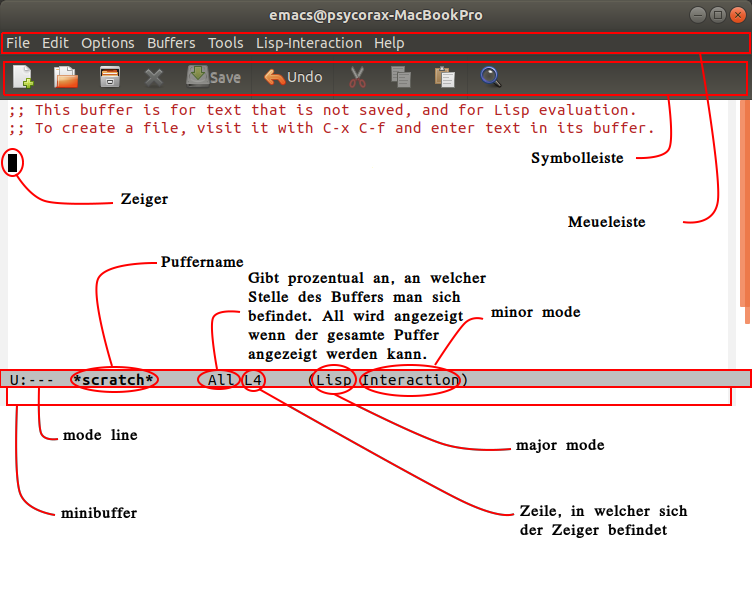
\includegraphics[width=.95\textwidth]{./images/Grundlagen/Emacsscreen.png}
  \caption{\label{fig:Emacsscr} Ein Emacs-Rahmen mit einem Fenster in
    der \textit{Default}-Konfiguration.}
\end{figure}

\section{Die Konfigurationsdatei}
\label{sec:konfdatgl}
Emacs kann an die persönlichen Anforderungen angepasst werden. Um
diese Anpassungen nicht für jede Sitzung neu vornehmen zu müssen,
geschieht dies in Form einer Konfigurationsdatei. Diese Datei wird bei
jedem Start von Emacs geladen. Ist keine Konfigurationsdatei
vorhanden, so startet Emacs mit den Standardeinstellungen. Emacs sucht
drei verschiedene Konfigurationsdateien unter \cite{EmacsInitfile}:
\begin{itemize}
\item $\sim$/.emacs
\item $\sim$/.emacs.d
\item $\sim$/.emacs.d/init.el
\end{itemize}
Das Tilde-Symbol {\glqq}$\sim${\grqq} kennzeichnet das
\textit{Home}-Verzeichnis.  Wenn eine dieser drei Dateien gefunden
wird, so wird diese zur Initialisierung verwendet. In dieser Arbeit
wird zur Konfiguration die Datei \textit{init.el} im Verzeichnis
\textit{$\sim$/.emacs.d/} verwendet.

In dieser Datei, können beliebig viele Konfigurationen vorgenommen
werden. Da sich Emacs nur anhand dieser Datei konfiguriert, kann auf
jedem Gerät Emacs mit den selben Einstellungen gestartet werden. Diese
Konfigurationen sind in der Programmiersprache \textit{Emacs Lisp}
(siehe Abschnitt \ref{sec:emacslisp}) geschrieben, was auch die Endung
{\glqq}el{\grqq} verrät.

Mögliche Konfigurationen sind:
\begin{itemize}
\item Anpassen der Tastenkombinationen an die eigenen Bedürfnisse,
\item Einstellungen, welche Modi wann aktiv sein sollen und generelle
  Konfigurationen an Modi,
\item Einstellen beliebiger Farbschemata und generell der
  Benutzeroberfläche,
\item Installieren zusätzlicher Pakete und
\item Definieren eigener Funktionen.\\
\end{itemize}
Der Aufbau der Konfiguration wie sie in dieser Arbeit durchgeführt
wird, ist nicht nur auf eine Datei beschränkt. Es können in der
verwendeten Datei \textit{init.el} weitere Dateien geladen
werden. Diese sind \textit{org}-Dateien. Durch die Auslagerung der
Konfigurationen auf diese \textit{org}-Dateien wird die Konfiguration
übersichtlicher.\\

\section{Pakete}
\label{sec:paketebasics}
Pakete sind Erweiterungen, welche zusätzliche Funktionalität für Emacs
implementieren. Es gibt Pakete, die standardmäßig installiert
sind. Diese sind in dem Archiv {\glqq}GNU{\grqq} vorhanden. Zusätzlich
zu diesen gibt es Pakete von der \textit{Community}. Das größte Archiv
in dem diese Pakete gesammelt werden ist
\textit{melpa}\footnote{\url{https://melpa.org/}}. Emacs bietet
einfache Möglichkeiten um Pakete zu installieren. Die Installation
kann direkt im \textit{minibuffer} erfolgen. Der Nachteil an dieser
Methode ist, dass bei einer Neuinstallation von Emacs diese Pakete
nicht mehr vorhanden sind. Eine Abhilfe schafft der Installationsweg
über eine Konfigurationsdatei. In dieser können alle beliebigen Pakete
angegeben werden, welche von Emacs beim Start geladen werden
sollen. Die verfügbaren Pakete können mittels \textbf{M-x
  package-list-packages} angezeigt werden. \\

\section{Emacs Lisp}
\label{sec:emacslisp}
Die Programmiersprache \textit{Emacs Lisp} ist ein Dialekt der
Programmiersprache \textit{Lisp}. \textit{Emacs} selbst ist zum
größten Teil in dieser Sprache programmiert. Aus diesem Grund werden
auch die Erweiterungen in dieser Sprache geschrieben. \textit{Emacs
  Lisp} arbeitet mit Listen und Listen von Listen. In \textit{Lisp}
wird alles in Form von Listen verarbeitet und abgespeichert. Das
bedeutet, Daten und Programme werden auf die gleiche Art
repräsentiert. Dadurch ist es sehr einfach ein Programm als ein Datum
für ein anderes Programm zu verwenden. Eine Liste wird definiert, in
dem alle Elemente der Liste zwischen Klammern geschrieben werden, die
einzelnen Elemente werden durch Leerzeichen getrennt. \cite{EmacsLisp}

Ein einfache Liste ist: {\glqq}(+ 2 3){\grqq}. Diese Liste besteht nun
aus einem Plus-Symbol, einer eins und einer zwei. Das erste Symbol der
Liste wird von dem System als Kommando interpretiert. Das Plus-Symbol
ruft ein Funktion zum Addieren auf. Diese Funktion lässt beliebig
viele Parameter zu. In diesem Fall sind es zwei Parameter. Die Liste
kann mit \textbf{C-x C-e} ausgeführt werden. Im \textit{minibuffer}
wird das Ergebnis {\glqq}5{\grqq} angezeigt. Sollte vor der Liste ein
Hochkomma {\glqq}'{\grqq} stehen, so wird beim Ausführen der Liste
nach keinem Kommando an erster Stelle gesucht. Derselbe Effekt wird
mit dem Begriff {\glqq}quote{\grqq} erzielt. Es wird die Liste einfach
so wie sie ist ausgegeben. Als Beispiel wird die Liste '(+ 2 3)
verwendet, welche dasselbe aussagt wie (quote(+ 2 3)). Nach Ausführen
der Liste wird im \textit{minibuffer} die Liste (+ 2 3) ausgegeben, da
das erste Element der Liste nicht als Kommando interpretiert wird. In
der angeführten Grafik \ref{fig:elisp}, sind beide Listen zu
sehen. Diese Listen wurden mit der Tastenkombination \textbf{C-j}
ausgeführt. Der Unterschied zwischen \textbf{C-x C-e} und \textbf{C-j}
ist, dass bei \textbf{C-j} das Ergebnis zusätzlich in den Puffer
geschrieben wird.\\

\begin{figure}[h]
  \centering
  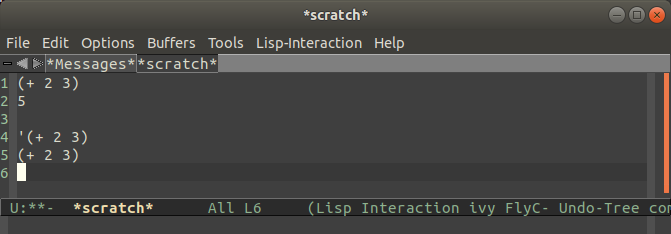
\includegraphics[width=.95\textwidth]{./images/Grundlagen/Elisp.png}
  \caption{\label{fig:elisp}Zweimal der selbe Inhalt in einer
    Liste. Einmal wurde die Liste mit voranstehendem Hochkomma und
    einmal ohne ausgeführt.}
\end{figure}

\section{Der Modus org}
\label{sec:orgmode}
Der \textit{org-mode} ist ein \textit{major-mode} in Emacs. Der Modus
dient zur Verarbeitung von Text und wird für folgende Aufgaben
verwendet:
\begin{itemize}
\item Zum Niederschreiben von Notizen,
\item Für das Erstellen von \textit{TODO-Listen} und
\item Zur Planung von Projekten.
\end{itemize}
Der \textit{org-mode} wird ebenfalls dazu verwendet, um
Programmiersprachen einfach und leserlich für Menschen
darzustellen. Der Modus ist ein einfach in der Verwendung und gut
geeignet für Einsteiger. Wird mehr Funktionalität benötigt, steht
diese ebenfalls zur Verfügung. \cite{OrgMode}

\textit{Org-mode} ist in Emacs standardmäßig enthalten, es kann jedoch
eine aktuellere Version installiert werden. Der Modus wird automatisch
verwendet, wenn eine Datei mit der Endung {\glqq}.org{\grqq} in einen
Puffer geladen wird. Der \textit{org-mode} kann auch manuell mit dem
Kommando \texttt{M-x org-mode} aktiviert werden.\\

\subsection{Die Installation von org-mode}
In dieser Arbeit wird die Version
\textit{org-elpa}\footnote{\url{https://orgmode.org/elpa.html}}
installiert. Es muss darauf geachtet werden, dass vor der Installation
in der Konfigurationsdatei keine \textit{org}-Funktion ausgeführt
wird. Aus diesem Grund erfolgt die Installation in der Datei
{\glqq}init.el{\grqq}, noch vor dem Laden der \textit{org}-Datei. Der
Grund warum \textit{org-mode} aktualisiert wird ist, dass die aktuelle
Version Text-Hervorhebung für \textit{org} Dateien innerhalb von
Code-Blöcken ermöglicht.\\

\subsection{Kapitel und Überschriften}
\label{subsec:kapitel}
\textit{Org} kann so wie \textit{Latex} mit Kapitel und
       {\glqq}Unterkapitel{\grqq} organisiert werden. Die Überschrift
       eines Kapitels beginnt mit einem Stern, gefolgt von einem
       Leerzeichen. Die Überschrift eines Unterkapitels hat zwei
       Sterne gefolgt von einem Leerzeichen, dies setzt sich so
       fort. Damit können {\glqq}Bäume{\grqq} aufgebaut werden. Unter
       diesen Überschriften kann jeder beliebige Inhalt stehen. Die
       Funktion \texttt{org-cycle} ist auf die Taste \textbf{TAB}
       gebunden, damit können die einzelnen Inhalte der Überschriften
       ein und ausgeblendet werden. Es gibt drei Zustände:
\begin{itemize}
\item \textbf{folded} : Alles bis auf die Überschriften der Kapitel
  ist sichtbar.
\item \textbf{children} : Alle Überschriften sind sichtbar.
\item \textbf{subtree} : Alle Überschriften und Inhalte sind sichtbar.
\end{itemize}
Ist der Inhalt einer Überschrift ausgeblendet, so wird dies durch drei
Punkte am Ende der Überschrift gekennzeichnet. Es gibt die Funktion
\texttt{org-global-cycle}. Diese ist auf die Tastenkombination
\textbf{<shift> TAB} gebunden. Diese besitzt ebenfalls drei
Zustände. Der Unterschied zu der Funktion \texttt{org-cycle} ist, dass
sie für alle Überschriften in der Datei gelten. Die Namen der Zustände
sind:
\begin{itemize}
\item \textit{OVERVIEW}
\item \textit{CONTENTS}
\item \textit{SHOW ALL}
\end{itemize}
Mit der Hilfe dieser Funktionalität von \textit{org} ist es einfacher,
den Überblick über große Dateien zu bewahren. In der folgenden Grafik
\ref{fig:headlines} sind dreimal die selben Kapitel mit der selben
Anzahl an Unterkapitel und selbem Inhalt in unterschiedlichen
Zuständen dargestellt. Es sind am Ende einiger Überschriften die drei
Punkte zu erkennen. Das Inhalt versteckt ist, ist auch den
Zeilennummern zu entnehmen.\\

\begin{figure}[h]
  \centering
  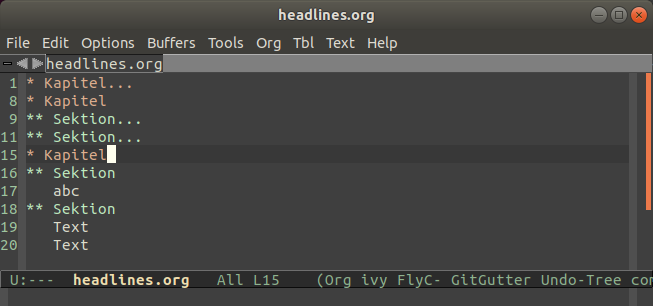
\includegraphics[width=.95\textwidth]{./images/KonfigurationUndPakete/headlines.png}
  \caption{\label{fig:headlines} Das erste Kapitel hat den Zustand
    {\glqq}folded{\grqq}. Das zweite Kapitel hat den Zustand
    {\glqq}children{\grqq}. Das dritte Kapitel hat den Zustand
    {\glqq}subtree{\grqq}.}
\end{figure}

Eine weitere Funktionalität ist, dass diese Kapitel und Unterkapitel
verschoben werden können. Dies kann mit den Pfeil-Tasten bei
gedrückter alt-Taste durchgeführt werden. Dazu muss sich der Zeiger
auf der zu verschiebenden Überschrift befinden. Die Reihenfolge der
Kapitel und Unterkapitel kann dadurch einfach verändert werden. Es
können Unterkapitel in andere Kapitel verschoben werden. Außerdem kann
auch ein Unterkapitel in der Hierarchie nach {\glqq}außen{\grqq}
geschoben werden, wodurch aus diesem Unterkapitel ganz einfach ein
eigenständiges Kapitel wird. Dadurch wird das Umstrukturieren der
Datei sehr einfach.

Es ist möglich, die Überschriften mit einem {\glqq}TODO{\grqq} oder
{\glqq}DONE{\grqq} zu versehen. Dies kann mit den Pfeil-Tasten bei
gehaltener shift-Taste durchgeführt werden. Dazu muss sich der Zeiger
auf einer Überschrift befindet.\\

\subsection{Makros}
\label{subsec:makro}
Beim Öffnen einer \textit{org}-Datei wird diese standardmäßig im
Zustand \textit{OVERVIEW} gezeigt. Ist dies nicht erwünscht, kann am
Anfang der Datei ein beliebiger Zustand mit Hilfe des Makros
\textit{\#+STARTUP} gesetzt werden. Die Möglichkeiten sind:
\begin{itemize}
\item \texttt{\#+STARTUP: overview}
\item \texttt{\#+STARTUP: content}
\item \texttt{\#+STARTUP: showall}
\item \texttt{\#+STARTUP: showeverything}
\end{itemize}
Der Zustand \textit{showeverything} zeigt zusätzlich auch die
versteckten Teile der Datei an. Die anderen Zustände wurden in
Abschnitt \ref{subsec:kapitel} bereits beschrieben.

Es gibt noch weitere vordefinierte Makros für den \textit{org-mode}
welche beim Exportieren von Dateien nützlich sind. Am häufigsten in
Verwendung sind:
\begin{itemize}
\item \textbf{\#+AUTHOR} : Der Name des Autors
\item \textbf{\#+DATE} : Datum
\item \textbf{\#+TITLE} : Titel der Datei
\item \textbf{\#+CAPTION} : Kurzbeschreibung
\end{itemize}

\subsection{Codeblöcke}
In \textit{org} können Codeblöcke eingefügt werden. Dies geschieht in
Form eines Makros (siehe Abschnitt \ref{subsec:makro}). Vor dem
Quellcode steht \texttt{\#+BEGIN\_SRC} und nach dem Quellcode steht
\texttt{\#+END\_SRC}. Alles was innerhalb dieser beiden Makros steht,
wird als Quellcode interpretiert. In der selben Zeile nach dem Makro
{\glqq}\texttt{\#+BEGIN\_SRC}{\grqq} kann einen Programmiersprache
definiert werden. Dadurch weiß Emacs welcher \textit{major-mode} zu
verwenden ist. Dies wird benötigt, damit die Formatierung und
Hervorhebung des Textes korrekt dargestellt werden kann. Der Codeblock
kann in \textit{org-mode} direkt mit der Tastenkombination \textbf{C-c
  C-c} evaluiert werden. Nach Ausführen des Codeblocks wird
automatisch das Makro \textit{\#+RESULT} erzeugt. Unterhalb dieses
Makros wird der Rückgabewert angegeben. Beispiele für einen
ausgeführten Emacs Lisp-Codeblock und einen Python-Codeblock folgen.\\

\lstinputlisting[language=Lisp, firstline=1,
  lastline=17]{./code/Pakete/Codeblock.org}

Codeblöcke mit Latex-Code sind sehr nützlich, wenn die Datei mittels
Latex exportiert wird (siehe Abschnitt \ref{subsec:export}). Dadurch
können Bilder, Tabellen oder mathematische Formeln wie gewohnt in
{\glqq}Latex{\grqq} geschrieben werden.\\

\subsection{Exportieren}
\label{subsec:export}
\textit{Org} kann Text in verschiedene {\glqq}Formate{\grqq}
exportieren. Die wichtigsten sind:
\begin{itemize}
\item Latex
\item PDF
\item HTML
\end{itemize}
Wenn eine PDF-Datei erzeugt werden soll, kann diese mittels Latex
exportiert werden. Das bedeutet, dass aus der \textit{org}-Datei eine
\textit{tex}-Datei erzeugt wird und diese dann zum Erzeugen einer
\textit{PDF-Datei} verwendet wird. \textit{Org}-Dateien können auch in
eine \textit{HTML}-Datei exportiert werden. Dadurch lassen sich
einfache Webseiten realisieren. Diese \textit{HTML}-Dateien eigenen
sich auch als einfache Präsentationen.\\

\subsection{Tabellen}
In \textit{org} können sehr einfach Tabellen erstellt werden. Spalten
werden mittels {\glqq}|{\grqq} unterteilt. Die oberste Reihe der
Tabelle gibt die Anzahl der Spalten vor. Darunter wird einfach
{\glqq}|-{\grqq} und die Tabulator-Taste gedrückt. Ein Beispiel einer
solchen Tabelle:\\

\lstinputlisting[language=Lisp, firstline=1,
  lastline=3]{./code/Pakete/Tabellen.org}

Nach dem Eintragen der Daten, passt die Tabelle automatisch die Größe
der Spalten und Zeilen an. Die Tabelle kann mit der Tastenkombination
\textbf{C-c C-c} manuell ausgerichtet werden. Die Spalten und Zeilen
können mit den Pfeiltasten bei gedrückter ALT-Taste vertauscht
werden. Die Tastenkombination \textbf{C-c \^} sortiert die Inhalte
einer Tabelle. In der folgenden Tabelle sind die Einträge alphabetisch
sortiert. Es ist ebenfalls erkennbar, dass sich die Spaltenbreite an
die längste Zeichenkette der Spalte angepasst hat.\\

\lstinputlisting[language=Lisp, firstline=4,
  lastline=10]{./code/Pakete/Tabellen.org}
